%-------------------------------------------------------
%	DOCUMENT CONFIGURATIONS
%-------------------------------------------------------
\graphicspath{{./annexes/}} % Defines path to the graphics for this page

%-------------------------------------------------------
%	START OF ANNEXES
%-------------------------------------------------------
\section{Annexes}
\todo[inline]{Add other crypto libraries using \textbf{Dominic Tarr}'s benchmark set \cite {Tarr2014PerformanceLibraries.}.}

\subsection{JS Cryptography Library Graphs}
\todo[inline]{TODO}
The graphs from the following figures have been made by \textbf{Dominic Tarr} \cite {Tarr2014PerformanceLibraries.}

\begin{figure}
\centering
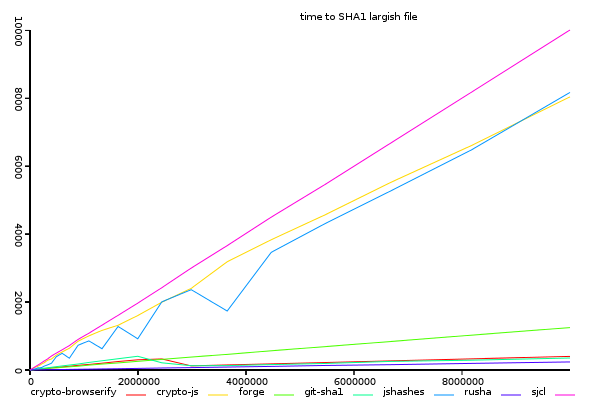
\includegraphics[scale=0.6]{graphs/hash-sha1.png}
\caption{\small \sl y-axis shows total time taken, lower is better
\label{fig:hash-sha1}}  
\end{figure}

\begin{figure}
\centering
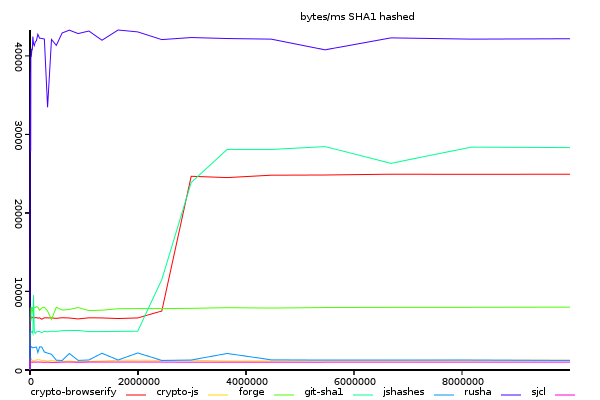
\includegraphics[scale=0.6]{graphs/hash-ops-sha1.png}
\caption{\small \sl y-axis shows size/time, higher is better
\label{fig:hash-ops-sha1}}
\end{figure}

\begin{figure}
\centering
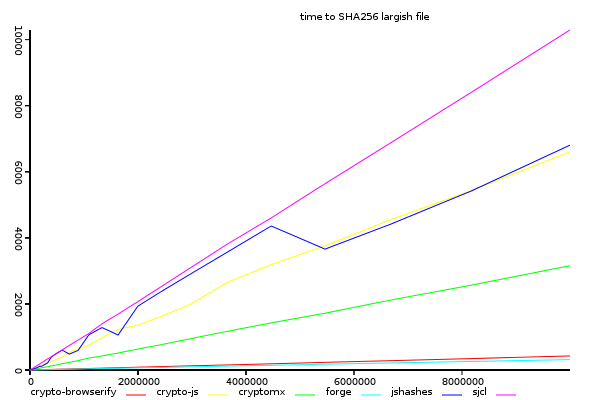
\includegraphics[scale=0.6]{graphs/hash-sha256.png}
\caption{\small \sl y-axis shows total time taken, lower is better
\label{fig:hash-sha256}}
\end{figure}

\begin{figure}
\centering
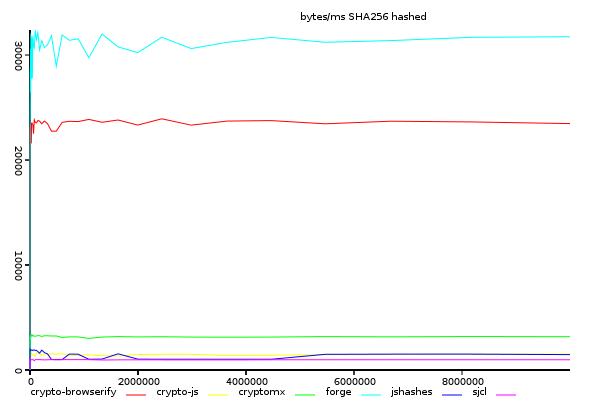
\includegraphics[scale=0.6]{graphs/hash-ops-sha256.png}
\caption{\small \sl y-axis shows size/time, higher is better
\label{fig:hash-ops-sha256}}
\end{figure} 

\begin{figure}
\centering
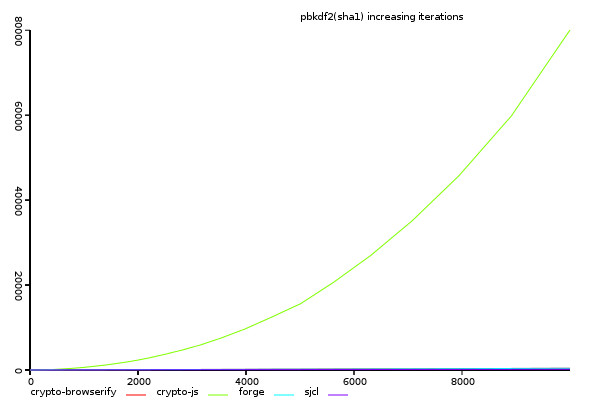
\includegraphics[scale=0.6]{graphs/pbkdf2-sha1.png}
\caption{\small \sl y-axis shows total time taken, lower is better
\label{fig:pbkdf2-sha1}}
\end{figure}

\begin{figure}
\centering
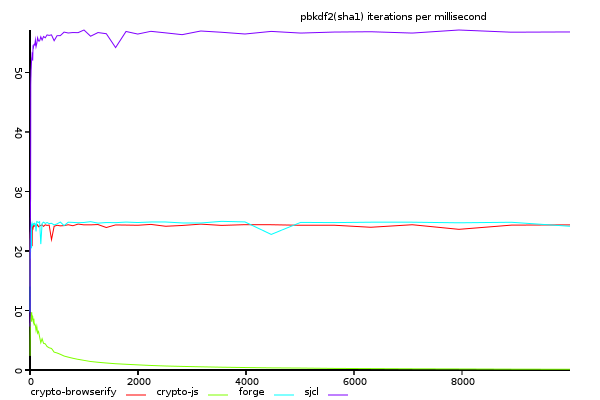
\includegraphics[scale=0.6]{graphs/pbkdf2-ops-sha1.png}
\caption{\small \sl y-axis shows size/time, higher is better
\label{fig:pbkdf2-ops-sha1}}
\end{figure}

\begin{figure}
\centering
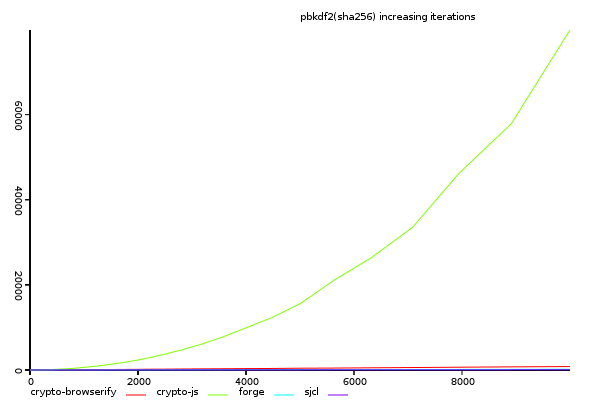
\includegraphics[scale=0.6]{graphs/pbkdf2-sha256.png}
\caption{\small \sl y-axis shows total time taken, lower is better
\label{fig:pbkdf2-sha256}}
\end{figure}

\begin{figure}
\centering
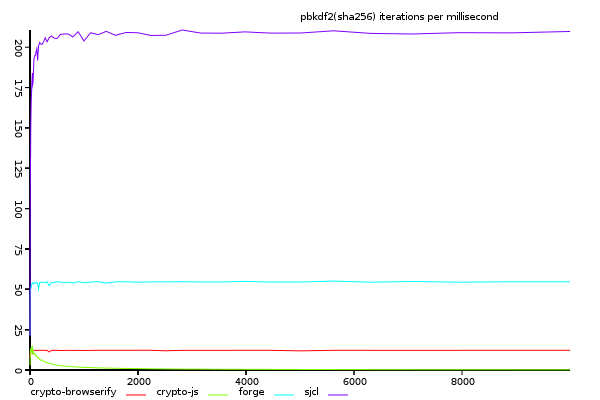
\includegraphics[scale=0.6]{graphs/pbkdf2-ops-sha256.png}
\caption{\small \sl y-axis shows size/time, higher is better
\label{fig:pbkdf2-ops-sha256}}
\end{figure}

\begin{figure}
\centering
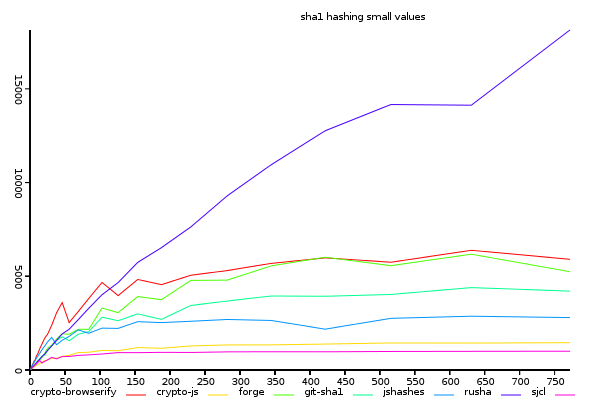
\includegraphics[scale=0.6]{graphs/small-hash-sha1.png}
\caption{\small \sl y-axis shows size/time, higher is better
\label{fig:small-hash-sha1}}
\end{figure}

\begin{figure}
\centering
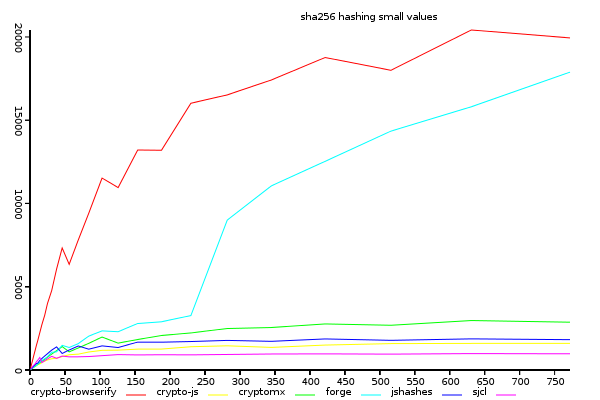
\includegraphics[scale=0.6]{graphs/small-hash-sha256.png}
\caption{\small \sl y-axis shows size/time, higher is better
\label{fig:small-hash-sha256}}
\end{figure}

\begin{figure}
\centering
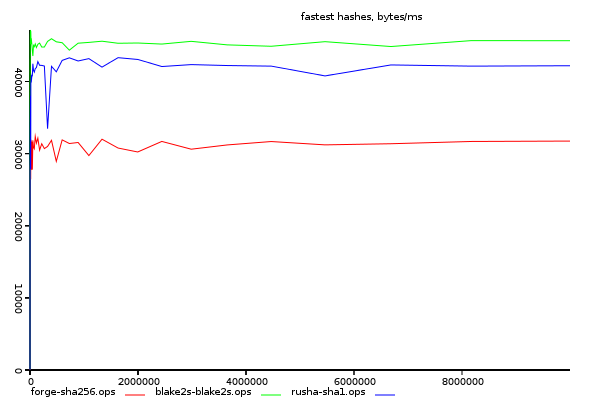
\includegraphics[scale=0.6]{graphs/hash-ops-best.png}
\caption{\small \sl y-axis size/time, higher is better
\label{fig:hash-ops-best}}
\end{figure} 

%-------------------------------------------------------
%	END OF ANNEXES
%-------------------------------------------------------